\vspace{10mm}

\noindent %Bu bölüm resim koymak içindir. Resim koymak istemiyorsanız, resim dosyasının tanımlandığı satırın başına "%" işareti koyabilirsiniz.
%Resim koymak istiyorsanız, kendi resminizin dosyasını "CV.jpg" olarak kaydetmeniz yeterlidir ve bu bu bölümde herhangi bir değişiklik yapmanıza gerek yoktur.

\newsavebox{\mysquare}
\savebox{\mysquare}{\textcolor{black}{\rule[2.3pt]{3.4pt}{3.4pt}}}

\setlength{\TPHorizModule}{10pt}
\setlength{\TPVertModule}{10pt}

\begin{textblock}{1}(40,10)
 	\begin{figure}[p]
        % Resim dosyasını burada tanımlayın. Resim girilmesi zorunlu değildir.
		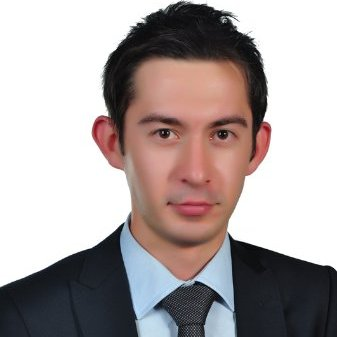
\includegraphics[width=3.5cm,keepaspectratio=true]{./fig/CV.jpg}
	\end{figure}
\end{textblock}

\noindent \textbf{Ad Soyad:} Ahmet Karabacak \\

\vspace{-3mm}
 \textbf{Doğum Tarihi ve Yeri:} 1993, Konya \\

\vspace{-3mm}
 \textbf{E-Posta:} ahmet7k@gmail.com \\

\textbf{ÖĞRENİM DURUMU:} \vspace{-3mm}

\begin{itemize}
\item \textbf{Lise:} 2011, Konya Atatürk Lisesi 
\item \textbf{Lisans:} 2016, Eskişehir Osmangazi Üniversitesi, İnşaat Mühendisliği 
\item \textbf{Y. Lisans:} 2019, İstanbul Teknik Üniversitesi, Deprem Mühendisliği
\end{itemize}
\textbf{MESLEKİ DENEYİMLER VE ÖDÜLLER:} \vspace{-3mm}

\begin{itemize}
\item Soyut İnşaat 2013-2016 ,Yarı-zamanlı mühendislik uygulamaları
\item 2014-2016 tarihlerinde Eskişehir Osmangazi Üniversitesi İnşaat Mühendisliği
bölüm temsilciliği
\item 2014 yılında TAV İnşaat Emaar Square projesinde saha stajı
\item 2015 yılında Alarko Holding merkez ofis, arazi geliştirme grubunda
ofis stajı
\item Erdemli Proje Müşavirlik 2016- Halen , Yapı Tasarım Mühendisi
\item Bu tez 42127 numaralı İTÜ Bilimsel Araştırma Projesi kapsamında kabul
edilmiştir.
\end{itemize}
% ---------------------------------------------------------------- %
% Fotografli ve yayin listeli (yayini varsa) ozgecmis onerilir.    %
% Fotograf ve adres sart degildir.                                 %
% -----------------------------------------------------------------%